% -*- coding: utf-8 -*-

\chapter{Estado del arte y trabajos relacionados}
\label{chap:antecedents}
\drop{E}{n} el siguiente capítulo se realiza una presentación de los conceptos y
tecnologías que han sido utilizadas para la elaboración del proyecto y se hace
un repaso de algunos de los trabajos y aplicaciones reales que han servido de
inspiración para el diseño final del sistema.

\section{Estado del arte}
A continuación, se citan los principales elementos que constituyen la base
teórica sobre la que se sustenta el resto del escrito.

  \subsection{La tecnología \acs{RFID}}
\acs{RFID} son las siglas de \emph{Radio Frequency IDentification} (en
castellano, \emph{\textbf{identificación por radiofrecuencia}}). Se trata de un
sistema de almacenamiento y recuperación de datos remoto que utiliza las ondas
de radio para transmitir la identidad (única) de un objeto.

El modo de funcionamiento de los sistemas \acs{RFID} es simple. Una
\textbf{etiqueta \acs{RFID}} (o transponedor) que contiene datos genera una
señal de radiofrecuencia con dichos datos. Esta señal es captada por un
\textbf{lector \acs{RFID}} y este la transforma a una señal digital entendible
por una aplicación específica que utilice \acs{RFID} (figura
\ref{fig:rfidSystem}).

\begin{figure}[!h]
  \begin{center}
    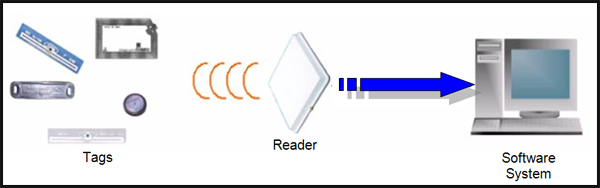
\includegraphics[width=0.8\textwidth]{rfidSystem.png}
    \caption{Esquema básico de un sistema \acs{RFID}.}
    \label{fig:rfidSystem}
  \end{center}
\end{figure}

    \subsubsection{Historia}
  El origen del \acs{RFID} está relacionado con la II Guerra Mundial. Los
  radares de la época eran capaces de detectar y medir la presencia de objetos
  dentro de un rango de actuación, pero no eran capaces de identificar qué
  clase de objetos eran identificados.

  Durante la década de los 50 y los 60, científicos de los países más
  avanzados, trabajaron para explicar cómo podrían identificar objetos
  remotamente. Fruto de estos estudios se inventaron los primeros sistemas
  antirrobo que funcionaban con ondas de radio. El objeto en cuestión tenía 
  una etiqueta con un único bit que decía si el artículo se había pagado o no.
  Cuando el objeto había sido pagado, se modificaba dicho bit, para que los 
  sensores de la salida no accionaran la alarma.

  Las primeras patentes fueron solicitadas en Estados Unidos en 1973. Mario W.
  Cardullo presentó una etiqueta \acs{RFID} activa que portaba una memoria
  rescribible. Y ese mismo año, Charles Walton recibió la patente para un
  sistema \ac{RFID} pasivo, consistente en una tarjeta con un transponedor que
  comunicaba una señal a un lector situado en una puerta. Si la tarjeta era
  validada por el lector, se desbloqueaba la cerradura de la puerta.

  A partir de ese año, la tecnología \acs{RFID} empezó a utilizarse por ejemplo,
  en sistemas de apertura de puertas automáticas en centrales nucleares o en
  sistemas para controlar el ganado que había sido vacunado y el que no.

  En la década de los 90, el desarrollo de nuevos materiales permitió
  reducir drásticamente el precio de las etiquetas. Este hecho favoreció
  que se potenciara el número de aplicaciones que utilizan esta tecnología.
  Es por ello que organismos internacionales empezaran a poner sus esfuerzos en
  desarrollar estándares en el uso de este tipo de etiquetas.

    \subsubsection{Etiquetas \acs{RFID}. Arquitectura y funcionamiento}
  Las etiquetas \acs{RFID} son dispositivos pequeños, similares a una pegatina,
  que pueden incorporarse a un objeto, un animal o una persona. 
  
  Todas las etiquetas \acs{RFID} tienen en común los siguientes elementos
  (figura \ref{fig:rfidComponents}):

  \begin{figure}[!h]
    \begin{center}
      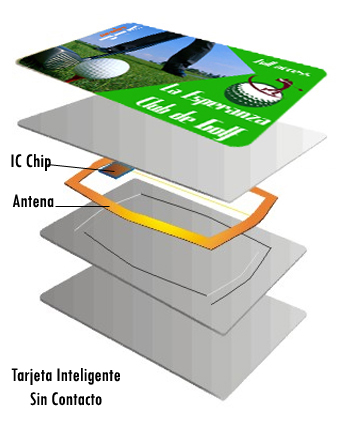
\includegraphics[width=0.4\textwidth]{rfidComponents.png}
      \caption{Componentes de una tarjeta \acs{RFID}.}
      \label{fig:rfidComponents}
    \end{center}
  \end{figure}

  \begin{itemize}
    \item \textbf{Antena}. Se encarga de recibir las señales emitidas por el
  lector y de enviar la respuesta ante dichas señales.
    \item \textbf{Chip}. Contiene la lógica de operación de la etiqueta y un
  número de identificación único.
    \item \textbf{Memoria}. Está compuesta por una parte de sólo lectura,
  que contiene las instrucciones básicas para el funcionamiento de la etiqueta;
  y por una parte de lectura y escritura, que almacena los datos escritos
  durante una comunicación con el lector.
  \end{itemize}
  
  Por otro lado, las etiquetas \ac{RFID} pueden ser de tres tipos:
  \begin{itemize}
    \item \textbf{Pasivas}. No poseen ninguna fuente autónoma de energía. La
  señal del lector es la que le induce una pequeña cantidad energía suficiente 
  como para generar y transmitir la respuesta. Tienen una fiabilidad y una
  capacidad de almacenamiento muy limitadas (unos pocos KBytes) y su campo de
  cobertura es también muy reducido (hasta 3 metros). Aún así, son las más
  utilizadas debido a su bajo coste.
   \item \textbf{Activas}. Poseen su propia fuente autónoma de energía y la
  utilizan para dar corriente a sus circuitos integrados y para propagar su
  señal al lector. Esto implica que las comunicaciones son más fiables (tienen
  menos errores), pueden transmitir señales más potentes y a mayor distancia
  (hasta 500m) y tienen más capacidad de almacenamiento. Por otro lado, tienen
  un mayor coste por chip y son de mayor tamaño que las etiquetas pasivas. La
  vida útil de sus baterías puede llegar hasta los 10 años.
    \item \textbf{Semipasivas}. Al igual que las etiquetas activas, las
  semipasivas también disponen de una fuente autónoma de energía. Sin embargo,
  estas utilizan la energía principalmente para alimentar el chip, no para
  transmitir la señal. Tienen una fiabilidad comparable a la de las etiquetas
  activas aunque superan su vida útil. Por otro lado, tienen un rango
  operativo comparable a las etiquetas pasivas aunque su respuesta es más
  rápida.
  \end{itemize}

    \subsubsection{Lectores RFID. Funcionamiento}
  Los lectores \acs{RFID} son los encargados de leer o re-escribir la
  información almacenada en las etiquetas.
  El funcionamiento es sencillo. La antena del lector crea un campo magnético
  y cuando este campo entra en contacto con una etiqueta, se produce la
  reacción de esta última, enviando al lector la información contenida.
  El lector decocifica los datos obtenidos y los manda a una tercera entidad 
  para que los interprete (figura \ref{fig:rfidSchema}).

  \begin{figure}[!h]
    \begin{center}
      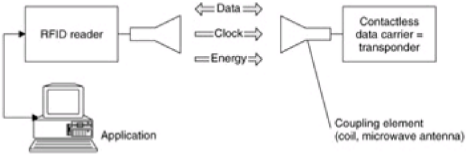
\includegraphics[width=0.8\textwidth]{rfidSchema.png}
      \caption{El lector y la etiqueta son los principales componentes de todo
sistema \acs{RFID}.}
      \label{fig:rfidSchema}
    \end{center}
  \end{figure}

  Según el número de bobinas que poseen, existen dos tipos de lectores:
  \begin{itemize}
  \item \textbf{Bobina simple}. La misma bobina crea el campo magnético y
  transmite los datos. Son más simples y baratas que las dobles y tienen
  un alcance muy limitado.
  \item \textbf{Bobina doble}. Una de las bobinas se encarga de crear el
  campo magnético y la otra de transmitir los datos. Son caras pero tienen
  mayores prestaciones que las bobinas simples.
  \end{itemize}
  
  En cuanto a la portabilidad, también existen dos tipos de lectores:
  \begin{itemize}
  \item \textbf{Lectores móviles}. Son lectores autónomos que pueden 
  transportarse a cualquier lugar y que pueden utilizarse con varios fines. Se
  comunican con otros dispositivos a través de conexiones inalámbricas.
  \item \textbf{Lectores fijos}. Son lectores ubicados en un punto fijo y 
  dedicados a un único fin. Tienen mayor rango de actuación que los lectores
  móviles y suelen utilizarse en sistemas de detección y seguimiento de
  personas y animales.
  \end{itemize}

%    \subsubsection{La tecnología \emph{MIFARE}}
%  \emph{MIFARE} es el estándar de la industria para interfaces de
%  tarjetas inteligentes sin contacto y lectores que operan a 13.56MHz.
%  Funcionan de acuerdo con el estándar \acs{ISO} 14443\cite{bib:mifare}.
  
%  El alcance típico de lectura/escritura de etiquetas \emph{MIFARE} sin
%  contacto oscila entre los 2 y los 10 cm; y la capacidad más habitual está
%  entre los 1 y los 4KB de memoria \acs{EEPROM}.

%  Para que los datos sean leídos o escritos es necesaria una autentificación 
%  mútua entre el lector y la etiqueta, ya que el acceso a los mismos está 
%  protegidos por una clave de 48 bits. La transmisión de datos por
%  radiofrecuencia viaja encriptada.

%  En la actualidad \emph{MIFARE} es una marca registrada de \emph{NXP
%  Semiconductors} (empresa fundada por \emph{Philips}). Ha vendido más de 5 mil
%  millones de tarjetas y etiquetas inteligentes y más de 50 millones de
%  componentes de lectores. Ha sido seleccionada para la mayoría
%  de proyectos importantes con tarjetas inteligentes sin contacto en todo el
%  mundo y su cartera de productos incluye soluciones perfectas para la
%  recaudación automática de tarifas, tarjetas de fidelización, cobro en 
%  carreteras de peaje o gestión de acceso a edificios\cite{bib:urlMifare} 
%  (figura \ref{fig:mifareFamily}).

%  \begin{figure}[!h]
%    \begin{center}
%      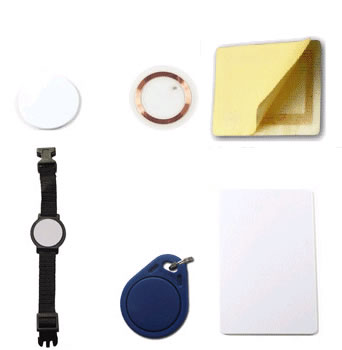
\includegraphics[width=0.5\textwidth]{mifareFamily.png}
%      \caption{Ejemplos de etiquetas MIFARE.}
%      \label{fig:mifareFamily}
%    \end{center}
%  \end{figure}

% El chorizo de las siguientes partes lo meteré más adelante...
  \subsection{La tecnología \acs{NFC}}
\acs{NFC} son las siglas en inglés de \emph{Near Field Communication}
(Comunicación de Campo Cercano). Se trata de una tecnología inalámbrica de
corto alcance y alta frecuencia que permite el intercambio de información
entre dos dispositivos próximos entre sí.

\acs{NFC} se basa en la tecnología \acs{RFID}, que opera a 13,56MHz y tiene
una distancia de funcionamiento típica de 4 cm. Es compatible con tarjetas
inteligentes sin contacto \emph{Mifare} y \emph{FeliCa} y tiene una tasa de
intercambio de datos de hasta 424 Kb/s.

Los estándares de \acs{NFC} están basados en la \acs{ISO} 14443 e incluyen
la \acs{ISO}/\acs{IEC} 18092 y otros estándares definidos específicamente por
el \emph{NFC Forum}\footnote{Organismo formado en 2004 por los creadores de
\acs{NFC} (\emph{Nokia}, \emph{Philips} y \emph{Sony}) y que busca promover
el uso de esta tecnología. Para ello, crea especificaciones de desarrollo,
para asegurar la interoperabilidad entre dispositivos y servicios, y trata
de educar al mercado acerca de la tecnología \acs{NFC}. Actualmente, el foro
cuenta con más de 160 miembros, incluyendo fabricantes, desarrolladores de
aplicaciones, instituciones de servicios financieros, etc.\cite{bib:nfcForum}}.

Según el propio \emph{NFC Forum}\cite{bib:nfcForum}:

\emph{``Una tecnología de conectividad basada en estándares como \acs{NFC},
armoniza las diversas tecnologías actuales sin contacto, lo que permite
generar soluciones actuales y futuras en áreas tales como:
\begin{itemize}
\item Control de acceso.
\item Electrónica de consumo.
\item Salud.
\item Recogida e intercambio de información
\item Sistemas de fidelización y cupones.
\item Pagos.
\item Transporte.
\end{itemize}
''}.

%Una de las principales ventajas de la tecnología \acs{NFC} en los
%dispositivos móviles es que pueden ser utilizados como un dispositivo de
%almacenamiento de información, como una unidad de cómputo y como un lector
%\acs{NFC}. Esto les permite, por ejemplo, leer los datos de una etiqueta para 
%después utilizarlos como entrada en un proceso que trabaje con información 
%previamente almacenada, como ocurre en los pagos mediante \acs{NFC}.

%Otras ventajas importantes de \acs{NFC} son\cite{bib:currentBenefits}:
%\begin{itemize}
%\item La tecnología es compatible con las estructuras existentes de \acs{RFID}.
%Es decir, etiquetas \acs{RFID} y tarjetas inteligentes sin contacto.
%\item Es fácil de usar, ya que los usuarios no necesitan tener ningún
%conocimiento sobre la tecnología. Todo lo que el usuario tiene que hacer es
%iniciar la comunicación mediante la unión o contacto de dos dispositivos.
%\item El alcance de transmisión es tan corto que, cuando el usuario separa los
%dispositivos, la comunicación se corta. Esto hace que la seguridad sea
%inherente. Si no hay ningún otro dispositivo cerca, no habrá más
%comunicaciones.
%\end{itemize}

  \subsubsection{Funcionamiento}
Como se comentó anteriormente, tecnología \acs{NFC} está basada en las
tecnologías de tarjetas inteligentes sin contacto y en la tecnología
\acs{RFID}. Por lo tanto, el esquema básico de funcionamiento está formado
por un lector y por una etiqueta (figura \ref{fig:readerTag}). El lector puede 
estar empotrado como parte de otro dispositivo como: un teléfono móvil, un PC, 
un electrodoméstico, etc. o simplemente puede tratarse de un lector fijo (que 
esté a su vez conectado, por ejemplo, a un PC).

  \begin{figure}[!h]
    \begin{center}
      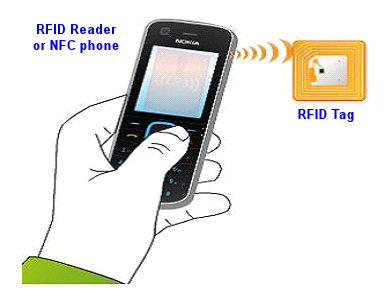
\includegraphics[width=0.4\textwidth]{readerTag.png}
      \caption{Ejemplo de interacción móvil \acs{NFC} - etiqueta.}
      \label{fig:readerTag}
    \end{center}
  \end{figure}

La interacción comienza cuando el lector se aproxima a una etiqueta
\acs{RFID}. Este emite una señal de corto alcance que es capaz de activar 
el microchip de la etiqueta y de hacer que emita los datos que contiene. En 
este caso el lector \acs{NFC} es siempre el que inicia la operación.

Pero también se permiten las comunicaciones entre dos lectores (figura
\ref{fig:mobileReader}). En este caso uno de los dos se encargará de iniciar y 
gestionar la comunicación. Existen dos modos de funcionamiento para los
dispositivos que cumplen el estándar \texttt{NFCIP-1}:

  \begin{figure}[!h]
    \begin{center}
      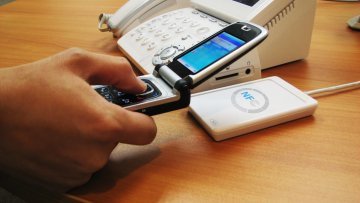
\includegraphics[width=0.5\textwidth]{mobileReader.png}
      \caption{Ejemplo de interacción móvil \acs{NFC} - lector \acs{NFC}.}
      \label{fig:mobileReader}
    \end{center}
  \end{figure}

\begin{itemize}
\item \textbf{Modo activo}:
En este modo, los dos dispositivos generan su propio campo magnético para
poder transmitir los datos. Es el modo característico de las comunicaciones
\acs{P2P} entre dispositivos (figura \ref{fig:activeMode}).

  \begin{figure}[!h]
    \begin{center}
      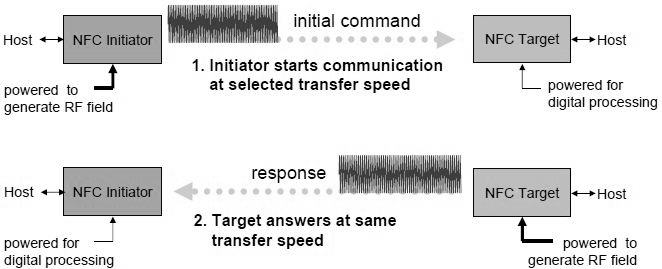
\includegraphics[width=0.8\textwidth]{activeMode.png}
      \caption{Esquema de funcionamiento del \emph{modo activo}.}
      \label{fig:activeMode}
    \end{center}
  \end{figure}

\item \textbf{Modo pasivo}:
Este modo es similar al esquema lector-etiqueta. Uno de los dispositivos
(el iniciador) genera el campo electromagnético necesario para activar al otro
y permitir la lectura de sus datos (figura \ref{fig:passiveMode}).

  \begin{figure}[!h]
    \begin{center}
      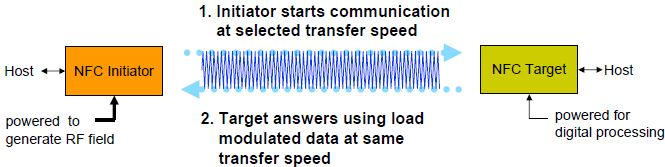
\includegraphics[width=0.8\textwidth]{passiveMode.png}
      \caption{Esquema de funcionamiento del \emph{modo pasivo}.}
      \label{fig:passiveMode}
    \end{center}
  \end{figure}
\end{itemize}

  \subsubsection{Características}

La tabla \ref{tab:nfcComparison} muestra una comparación entre 
las características de la tecnología \acs{NFC} y las características de 
otras tecnologías inalámbricas:

\begin{sidewaystable}[hp]
  \centering
  {\footnotesize
  \begin{tabular}{p{.12\textwidth}p{.12\textwidth}p{.12\textwidth}p{.12\textwidth}
                p{.12\textwidth}p{.12\textwidth}p{.12\textwidth}}
  \tabheadformat
  \tabhead{}   &
  \tabhead{\acs{NFC}}      &
  \tabhead{\acs{RFID}} &
  \tabhead{\acs{WiFi}} &
  \tabhead{\texttt{Bluetooth}} &
  \tabhead{\texttt{ZigBee}} &
  \tabhead{\acs{IrDA}} \\
\hline
\textit{Estándar}      & \acs{ISO}/\acs{IEC} 18092 & \acs{ISO}/\acs{IEC} 14443
                       & \acs{IEEE} 802.11         & \acs{IEEE} 802.15.1
                       & \acs{IEEE} 802.15.4       & \acs{IrDA} \\
\hline
\textit{Tasa de transferencia}
                       & 106-424 Kbps              & 106-424 Kbps
                       & 11-200 Mbps               & 1-480 Mbps
                       & 20-250 Kbps               & 1 Kbps - 100 Mbps \\
\hline
\textit{Frecuencia de utilización}
                       & 13.56 MHz                 & 13.56 MHz
                       & 2.4, 5.25, 5.6, 5.8 GHz   & 2.4 GHz
                       & 868/915 MHz, 2.4 GHz      & \\
\hline
\textit{Nº máximo de dispositivos que pueden interactuar}
                       & 2                         & 2
                       & Indefinida                & 8
                       & Indefinida                & 2 \\
\hline
\textit{Tiempo de inicialización}
                       & $<$ 0.1 ms                 & $<$ 0.1 ms
                       & $<$ 0.1 ms                 & 6 s
                       & $<$ 0.1 ms                 & 0.5 ms \\
\hline
\textit{Alcance}
                       & $<$ 20 cm                 & $<$ 3 m
                       & $<$ 100 m                 & $<$ 30 m
                       & $<$ 500 m                 & $<$ 5 m \\
\hline
\textit{Seguridad}
                       & Dada por la cercanía entre dispositivos
                       & Dada por la cercanía entre dispositivos
                       & Determinada por los mecanismos de encriptación     
                       & Determinada por los mecanismos de encriptación
                       & Determinada por los mecanismos de encriptación
                       & Dada por la cercanía entre dispositivos en línea recta \\
\hline
\textit{Consumo de energía}
                       & Mínimo o inexistente
                       & Mínimo o inexistente
                       & Alto para dispositivos alimentados por baterías
                       & Alto para dispositivos alimentados por baterías
                       & Muy bajo
                       & Bajo \\
\hline
\textit{Objetivo}
                       & Simplificar la interacción entre dispositivos
                         electrónicos          
                       & Realizar seguimiento de objetos y control de acceso
                       & Reemplazar cables en redes extensas, como las
                         \acs{LAN}
                       & Reemplazar cables para conectar dispositivos
                         electrónicos cercanos
                       & Control y monitoreo inalámbrico
                       & Reemplazar cables para conectar dispositivos
                         electrónicos cercanos \\
\hline
\textit{Ejemplo de aplicación}
                       & Intercambio de tarjetas personales electrónicas
                         acercando dos móviles
                       & Control de inventario en un supermercado
                       & Conexión entre dispositivos de una oficina (PCs,
                         impresoras, portátiles, etc.)
                       & Conexión de periféricos (teclado, ratón, etc.) a un
                         PC en la misma habitación
                       & Manejo de sistemas de riego usando sensores que
                         accionan los mecanismos correspondientes
                       & Transferencia de archivos entre un móvil y un PC \\
\hline
\end{tabular}


% Local variables:
%   coding: utf-8
%   ispell-local-dictionary: "castellano8"
%   TeX-master: "main.tex"
% End:

  }
  \caption[Comparativa entre tecnologías inalámbricas]
  {Comparativa entre tecnologías inalámbricas (\cite{bib:nfcComparison})}
  \label{tab:nfcComparison}
\end{sidewaystable}

Como se ha comentado anteriormente, una de las principales características de 
las conexiones \acs{NFC} es que su radio de acción es muy pequeño. Esto le
permite tomar parte en operaciones que necesitan mantener seguridad en la
privacidad de los datos, como por ejemplo, para el pago de servicios. El
hecho de que el dispositivo tenga que aproximarse al terminal de pago, evita
que pueda producirse de forma accidental, que entre en conflicto con otros
terminales cercanos o que la información que se transfiere de un dispositivo
a otro pueda ser observado por un tercero.

Por otro lado, las interacciones con \acs{NFC} son rápidas e intuitivas, ya 
que estas se producen  simplemente al aproximar el dispositivo a una etiqueta 
\acs{RFID} o a otro dispositivo. Dependiendo del contenido de estos, las 
interacciones generarán acciones más complejas automáticamente en el 
dispositivo como: el inicio de una aplicación, la generación de un evento 
dentro de la aplicación, el visionado del propio contenido, el envío de un 
mensaje automático, la solicitud de un servicio a través de otro medio de 
comunicación, etc.

  \subsubsection{Aplicaciones}
La creciente expansión de la tecnología \acs{NFC} ha provocado el desarrollo
de múltiples aplicaciones, que buscan aprovechar las características que esta 
tecnología les ofrece para solucionar o facilitar la realización de tareas 
cotidianas.

Existe un gran número de aplicaciones, pero todas ellas pueden agruparse en
una de estas tres categorías \cite{bib:nfcComparison}:
\begin{itemize}
\item \textbf{Inicialización de servicios}: 
En este tipo de aplicaciones, cuando un usuario toca con su dispositivo
\acs{NFC} una etiqueta \acs{RFID}, el lector extrae una serie de datos
(texto, \acs{URL}, número de teléfono, etc.) que le permiten realizar alguna
acción. Ejemplos de este tipo de aplicaciones son:
  \begin{itemize}
  \item Carteles inteligentes que promocionan un producto, servicio o evento. 
  En este caso las etiquetas proporcionan al usuario la \acs{URL} donde puede 
  obtener más información acerca de esa promoción.
  \item Etiquetas en los productos de un comercio que ofrecen más información
  acerca de dicho producto.
  \item Etiquetas ubicadas en los muebles de la casa para realizar acciones
  como controlar la iluminación o la temperatura a través del dispositivo
  móvil.
  \item Etiquetas que registran el número de visitas efectuadas por el
  personal de guardia a medida que hace el recorrido rutinario por las zonas
  del lugar.
  \item Etiquetas que facilitan operaciones simples a usuarios con alguna
  discapacidad física o mental. Por ejemplo, se puede confeccionar una agenda
  a partir de fotos de familiares a las que se adhiere una etiqueta con la
  información del número de teléfono. De esta forma cuando el usuario quiere
  llamar a alguno de sus familiares, sólo necesitará aproximar su dispositivo
  a la foto del familiar con el que quiere hablar.
  \end{itemize}
\item \textbf{Peer-to-peer}:
Este tipo de aplicaciones utilizan \acs{NFC} como mecanismo para establecer
la comunicación entre dos dispositivos que pretenden intercambiar datos. El
tráfico de dichos datos se podrá realizar mediante \acs{NFC} o mediante otra
tecnología inalámbrica (dependiendo del volumen de datos a transmitir).
Algunas de las aplicaciones que pertenecen a esta categoría son:
  \begin{itemize}
  \item Transmisión de fotos desde una cámara digital a una impresora. Cuando
  la cámara de fotos se aproxima a la impresora, se establece una comunicación
  \emph{Bluetooth} en la que el primer dispositivo le transmite las fotos al
  segundo.
  \item Intercambio de tarjetas personales electrónicas entre dos dispositivos
  mediante la aproximación de ambos.
  \item Configuración automática de una conexión \acs{WiFi} en un lugar
  público. El usuario aproxima su dispositivo a una etiqueta que contiene la
  configuración de red y utiliza estos parámetros para iniciar automáticamente
  una conexión \acs{WiFi}.
  \end{itemize}
\item \textbf{Compras y pagos}:
Este tipo de aplicaciones dio origen a los estándares \acs{NFC}. Como ya
existían tarjetas inteligentes sin contacto para realizar pequeñas
transacciones comerciales, la tecnología \acs{NFC} tuvo que ser definida
teniendo en cuenta que fuera compatible con las aplicaciones ya existentes.
Algunos ejemplos de estas aplicaciones son:
  \begin{itemize}
  \item Pagos en parquímetros y párkings.
  \item Pago en máquinas expendedoras.
  \item Consulta de saldo en tarjetas de transporte que utilizan \acs{NFC}.
  \item \emph{Monedero electrónico}. El objetivo final es que esta tecnología
  vaya sustituyendo a las tarjetas de plástico tradicionales. De esta forma
  el usuario de un dispositivo móvil con \acs{NFC} no sólo puede utilizar su
  dispositivo para pagar en un establecimiento, sino que también puede
  mantener la información de algún sistema de fidelización o puntos de dicho
  establecimiento, los datos de la tarjeta de la seguridad social, los datos
  de los bonos del sistema de transportes de su ciudad, etc. y todo ello
  accesible a través de la tecnología \acs{NFC}.
  \end{itemize}
\end{itemize}

El número de aplicaciones sigue creciendo y cada día son más las ciudades
que disponen de servicios accesibles a través de \acs{NFC}, sobretodo en
sitios como Japón, Corea del Sur o Estados Unidos. Los fabricantes de
dispositivos móviles han observado este hecho y año tras año han ido
sacando al mercado nuevos dispositivos que incluyen esta tecnología.
Como muestra la figura \ref{fig:nfcGraph} el porcentaje de los nuevos
dispositivos que cuentan con esta tecnología se ha ido incrementando
exponencialmente.

  \begin{figure}[!h]
    \begin{center}
      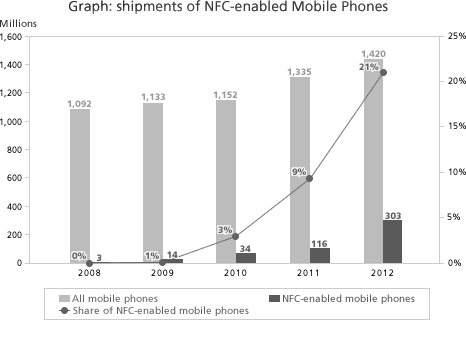
\includegraphics[width=0.8\textwidth]{nfcGraph.png}
      \caption{Evolución del número de teléfonos móviles que
      incorporan \acs{NFC}.}
      \label{fig:nfcGraph}
    \end{center}
  \end{figure}

El anexo \ref{chap:nfcMobiles} muestra una lista de los últimos dispositivos
que incluyen la tecnología \acs{NFC} entre sus características.

  \subsubsection{El formato \acs{NDEF}}
\acs{NDEF} (\acs{NFC} Data Exchange Format) es un formato definido por el
\emph{NFC Forum} y constituye el principal estándar para el intercambio y
almacenamiento de información, pues es un formato soportado por cualquiera 
dispositivo \acs{NFC}.

La estructura seguida por \acs{NDEF} posee una cabecera de datos, a partir de
la cual se encuentran los bloques de información. Cada bloque de información
se agrupa en registros que contienen a su vez los datos agrupados en mensajes
\acs{NDEF} y están caracterizados por un tipo \acs{MIME} definido. El
anexo \ref{chap:ndef} muestra un ejemplo de organización \acs{NDEF}.

Este formato tiene el inconveniente de que puede ser leido o modificado por
cualquier dispositivo \acs{NFC}, puesto que la clave empleada para el acceso
a los datos es la clave por defecto ($FF FF FF FF FF FF$, en hexadecimal).
Para solventar este problema, el formato \acs{NDEF} puede ser combinado con
el propuesto por \emph{MiFare}.

  \subsection{La tecnología \emph{Bluetooth}}
Bluetooth es el nombre común que se le da a la especificación industrial IEEE
802.15.1, que define un estándar global de comunicación inalámbrica que 
posibilita la transmisión de voz y datos entre diferentes dispositivos 
mediante un enlace por radiofrecuencia segura.

  \subsubsection{Historia}
Su nombre procede del nombre del rey danés y noruego Harald Blatan;
especialmente porque su traducción al inglés sería Harold Bluetooth, 
conocido por buen comunicador y por unificar las tribus noruegas, suecas y 
danesas.

En 1994, la compañía Ericsson inició diversas investigaciones con el 
objetivo de estudiar la viabilidad de la existencia de una nueva interfaz de 
comunicación, de bajo consumo y coste, entre diversos dispositivos como 
teléfonos móviles. Con todo ello, en el año 1999 se creó el SIG de Bluetooth 
(Special Interest Group), que consistía en la unión de diversas empresas 
(Ericsson, Intel, Nokia, Toshiba e IBM), e incorporándose a lo largo de
los años otras tantas (Microsoft, 3Com, Motorola, Lucent,...).

Se consiguió que los estudios iniciados avanzaran, y que los proyectos 
fueran de por sí una verdadera y auténtica realidad, consiguiendo extender 
el Bluetooth como un estándar para la interfaz aérea.

Técnicamente, la especificación Bluetooth definiría un canal de comunicación 
de máximo 720Kb/s con un alcance de 10m (llegando a los 100m con 
repetidores). La frecuencia de tráfico con la que trabaja, se encuentra en 
el rango de 2,4 a 2,48GHz con amplio espectro y saltos de frecuencia con 
posibilidad de transmitir en Full-Duplex3 con un máximo de 1600 saltos/s, 
los cuales se dan entre un total de 79 frecuencias con intervalos de 1Mhz.

Por todo, la potencia de salida para transmitir a una distancia máxima de 
10m es de 0dbm (1mW), mientras que la versión de largo alcance transmite 
entre los 20 y 30 dbm (entre 100mW y 1W).

Los principales objetivos que se pretenden alcanzar con esta norma son:
\begin{itemize}
\item Facilitar las comunicaciones entre dispositivos móviles y fijos.
\item Eliminar cables y conectores entre estos.
\item Ofrecer la posibilidad de crear pequeñas redes wireless y facilitar la
sincronización de datos entre equipos.
\end{itemize}

Desde sus comienzos hasta nuestros días, han existido distintas versiones en 
la tecnología Bluetooth a saber: v1.1, v1.2, v2.0 y la reciente v2.1 que 
promete simplificación en la configuración, menor consumo e incluso la 
combinación con otras tecnologías y protocolos como NFC.

  \subsubsection{La interfaz \emph{Bluetooth}}
Los productos Bluetooth de primera generación tenían como objetivo los 
entornos de negocio concretamente destinados a gente de negocios que viaja 
frecuentemente. Por lo que había que integrar el chip de radio Bluetooth en 
dispositivos móviles como Notebooks, teléfonos móviles, PDAs, auriculares... 
Esto originaba una serie de aspectos previos que deberían solucionarse:
\begin{itemize}
\item El sistema debería operar en todo el mundo.
\item El emisor de radio deberá consumir poca energía, ya que debe 
integrarse en equipos alimentados por baterías.
\item La conexión deberá soportar voz y datos, y por tanto aplicaciones 
multimedia.
\end{itemize}

\begin{description}
\item[La banda de frecuencia libre].
Para poder operar en todo el mundo es necesario disponer de una banda de
frecuencia abierta a cualquier sistema de radio independientemente del lugar 
del planeta donde nos encontremos. Hasta ahora, solo la banda ISM (médico-
científica internacional) de 2,45 Ghz cumple con éste requisito, con rangos 
que van de los 2.400 Mhz a los 2.500 Mhz, y solo con algunas restricciones 
en países como Francia, España y Japón.
\item[Salto de frecuencia].
Debido a que la banda ISM es abierta, el sistema de radio Bluetooth deberá 
estar preparado para evitar las múltiples interferencias que se pudieran 
ocasionar. Éstas pueden ser evitadas utilizando un sistema que busque una 
parte no utilizada del espectro o un sistema de salto de frecuencia. En los 
sistemas de radio Bluetooth se suele utilizar el método de salto de 
frecuencia debido a que ésta tecnología puede ser integrada en equipos
de baja potencia y reducido coste. Éste sistema divide la banda de 
frecuencia en varios canales de salto, donde, los transceptores, durante la 
conexión van cambiando de uno a otro canal de salto de manera pseudo-
aleatoria. Con esto se consigue que el ancho de banda instantáneo sea muy 
pequeño y también una propagación efectiva sobre el total de ancho de banda. 
En conclusión, con el sistema FH (Salto de frecuencia), se pueden conseguir 
transceptores de banda estrecha con una gran inmunidad a las interferencias.
\item[Definición de canal].
Bluetooth utiliza un sistema FH/TDD (salto de frecuencia/división de tiempo
duplex), en el que el canal queda dividido en intervalos de 625 $\mu$s, 
llamados slots, donde cada salto de frecuencia es ocupado por un slot. Esto da 
lugar a una frecuencia de salto de 1600 veces por segundo, en la que un 
paquete de puede ocupar un slot para la emisión y otro para la recepción y que 
pueden ser usados alternativamente, dando lugar a un esquema de tipo TDD.
Dos o más unidades Bluetooth pueden compartir el mismo canal dentro de una
piconet 4 , donde una unidad actúa como maestra, controlando el tráfico de 
datos en la piconet que se genera entre las demás unidades, que actúan como 
esclavas, enviando y recibiendo señales hacia la unidad maestra. El salto de 
frecuencia del canal está determinado por la secuencia de la señal, es 
decir, el orden en que llegan los saltos y por la fase de ésta secuencia. En 
Bluetooth, la secuencia queda fijada por la identidad de la unidad maestra 
de la piconet (un código único para cada dispositivo), y por su frecuencia 
de reloj. Por lo que, para que una unidad esclava pueda sincronizarse con 
una unidad maestra, ésta primera debe añadir un ajuste a su propio reloj 
nativo y así poder compartir lamisma portadora de salto.
\item[Definición de paquete].
La información que se intercambia entre dos unidades Bluetooth se realiza
mediante un conjunto de slots que forman un paquete de datos. Cada paquete 
comienza con un código de acceso de 72 bits, que se deriva de la identidad 
maestra, seguido de un paquete de datos de cabecera de 54 bits. Éste 
contiene importante información de control, como tres bits de acceso de 
dirección, tipo de paquete, bits de control de flujo, bits para la 
retransmisión automática de la pregunta, y chequeo de errores de campos de 
cabecera.
Finalmente, el paquete que contiene la información, que puede seguir al de 
cabecera, tiene una longitud de 0 a 2745 bits. En cualquier caso, cada 
paquete que se intercambia en el canal está precedido por el código de 
acceso. 
\item[Interferencias y seguridad].
Como ya se ha dicho, Bluetooth opera en una banda abierta y por lo tanto 
sujeta a considerables interferencias. A lo largo de las versiones de 
Bluetooth, el sistema ha sido optimizado para disminuir y evitar estas 
interferencias. Mediante técnicas de salto de frecuencias y reducción de 
ruido se ha conseguido disminuir considerablemente las interferencias 
producidas.
Por último, dado que los datos viajan de forma inalámbrica por el medio, en 
este caso el aire, es importante asegurar la protección de dicha 
información. Para ello queda definido un nivel básico de encriptación, que 
se ha incluido en el diseño del chip de radio para proveer de seguridad en 
equipos que carezcan de capacidad de procesamiento, donde las principales 
medidas de seguridad son:
\begin{itemize}
\item Una rutina de pregunta-respuesta para autenticación.
\item Una corriente cifrada de datos para encriptación.
\item Generación de una clave de sesión (con posibilidad de ser cambiada 
durante la conexión).
\end{itemize}
En los distintos algoritmos de seguridad del Bluetooth se usan tres objetos: 
la dirección de la unidad Bluetooth, como entidad pública; una clave de 
usuario privada, como entidad secreta; y un número aleatorio, que es 
diferente en cada nueva transacción.
Así, la dirección Bluetooth se obtiene a través de un proceso de consulta. 
La clave privada se obtiene durante la inicialización. Por su parte, el 
número aleatorio se genera en un proceso pseudo-aleatorio en cada unidad 
Bluetooth.
\item[Desventajas].
Una vez visto como funciona y los objetivos que persigue la tecnología 
Bluetooth (todos ellos tratados como ventajas de este tipo de conexión), y 
aunque se han dejado intuir las distintas desventajas de este protocolo, es 
en este punto donde se mencionarán de forma concisa dichas desventajas. 
Estas son:
\begin{itemize}
\item Velocidad de transmisión lenta para la transferencia de archivos de 
tamaño considerable (1MB/s). No obstante, las nuevas especificaciones tratan 
de aumentar su velocidad a 100MB/s.
\item Cuando es usado inadecuadamente el usuario del dispositivo puede ser
víctima de ataques (bluejaking).
\item Radio de alcance limitado entre los dispositivos. Más allá de dicho 
alcance no se garantiza la adecuada transmisión de los datos.
\item Limitación entre la cantidad de periféricos que podemos usar (p.e: los
adaptadores Bluetooth solo permiten un máximo de 7 equipos “pareados”).
\item Elevado consumo de la batería del dispositivo cuando el Bluetooth se
encuentra activado y en modo visible.
\end{itemize}
% Conexión SPP con javax.bluetooth (permite InputStream y OutputStream)

\end{description}

  \subsection{Los servicios web}
El World Wide Consortium lo define como “...un sistema software diseñado para
soportar interacción interoperable máquina a máquina sobre una red”.
Todo servicio web tiene una interfaz descrita en un formato procesable por una
máquina (WSDL 6 ) y las solicitudes de llamamiento a los servicios web se 
realizan utilizando mensajes SOAP 7 , típicamente enviados mediante HTTP. (W3C 
Consortium, 2004)
The Organization for the Advancement of Structured Information Standards y el
W3C son los responsables de la estandarización y arquitectura de los servicios 
web.
Al conjunto de servicios y protocolos para el manejo e implementación de los
servicios web se le conoce como “Web Services Protocol Stack” y básicamente son
utilizados para definir, localizar, implementar y hacer que un servicio web 
interactúe con otro. Este conjunto está conformado esencialmente de 4 
subconjuntos (Van de Putte, 2004):
\begin{itemize}
\item \textbf{Servicio de transporte}. Encargado del transporte de los 
mensajes entre aplicaciones sobre la red. Incluye varios protocolos del nivel 
de aplicación, siendo HTTP el más usado. Otros son: FTP, SMTP, BEEP y JMS.
\item \textbf{Mensajería XML}. Es el conjunto encargado de la codificación de 
los mensajes en XML estándar, pudiendo ser así interpretado en cualquiera de
los nodos de la red.
\item \textbf{Descripción del servicio}. El servicio web debe contar con una 
interfaz pública la cual es descrita en un formato denominado WSDL. WSDL es un
tipo de documento XML que describe lo que hace un servicio web, dónde se
encuentra y la forma de ser invocado. Este provee información muy
importante para los desarrolladores, describiendo el formato de los mensajes
que utiliza y a cuales puede responder.
\item \textbf{Descubrimiento de servicios}. El UDDI8 es un marco independiente 
de la plataforma para describir servicios, negocios e integrar servicios de
negocios. La estructura de UDDI está basada sobre los servicios estándares
de la web, lo que quiere decir que UDDI es accesible como otros servicios
web.
\end{itemize}

  \subsubsection{Arquitectura Orientada a Servicios (SOA)}
Es la arquitectura de servicios web más difundida. SOA es un modelo
arquitectónico de software creado y usado para diseñar modelos de negocio 
empaquetados como servicios. Dar una solución SOA exige un diseño aplicando 
los conceptos SOA, para lo cual es necesaria la utilización de un conjunto 
de herramientas de software, tecnologías y plataformas específicas. (Anantha 
Rangachar, 2006)
El enfoque de esta arquitectura hace que todo modelo de los servicios web 
gire en torno a los negocios. Siendo SOA uno de los logros de la ingeniería 
del software actual.
Muchos autores definen la arquitectura como “una unidad de código ejecutable 
que provee un encapsulamiento de caja negra física de servicios 
relacionados. Sus servicios pueden ser únicamente accedidos por una interfaz 
pública consistente, que incluye una interacción estándar. Un componente 
debe ser capaz de ser conectado con otros componentes para un largo grupo”. 
(Allen, 1998) Una arquitectura orientada a servicios es descrita como un 
conjunto de servicios que apuntan a los negocios, que son combinados para 
cumplir con los objetivos del negocio. Las Tecnologías de la Información y 
las Comunicaciones permiten, a través de sus herramientas, cumplir con 
dichos objetivos.
Por otra parte, una arquitectura orientada a servicios es una forma de 
arquitectura de sistemas distribuidos caracterizada por las siguientes 
propiedades: (W3C Consortium, 2004)
\begin{itemize}
\item \textbf{Vista lógica}. Proporciona una imagen de los componentes del 
sistema tales como bases de datos, procesos, programas,... explicando qué 
hace cada uno de ellos, normalmente llevándolos a la operación del nivel de 
negocio.
\item \textbf{Orientación al mensaje}. Se define el servicio en términos de 
los mensajes intercambiados por el agente solicitante y el agente proveedor. 
Se abstraen numerosos detalles. SOA solo se preocupa de los detalles 
expuestos en la descripción del servicio.
\item \textbf{Orientación a la descripción}. Un servicio web es descrito por 
metadatos procesables por una máquina. La descripción debe soportar la 
naturaleza pública de la SOA. La semántica del servicio debe quedar 
completamente definida.
\item \textbf{Granularidad}. Los servicios deben tender a realizar un 
pequeño número de operaciones con una gran cantidad de mensajes.
\item \textbf{Orientación a la red}. Los servicios web deben ser concebidos 
para ser usados sobre una red, aunque no sea un requerimiento necesario.
\item \textbf{Plataforma neutral}. Los mensajes deben ser creados para una 
plataforma neutral, utilizando un lenguaje estándar (XML) a través de las 
interfaces.
\end{itemize}

%  \subsection{El framework .NET}
%%%%%%%%%%%%%%%%%%%%%%%%%%%%%%
% No sé si meterlo

  \subsection{La tecnología \texttt{Java}}
La tecnología JAVA constituye una plataforma informática presentada por Sun
Microsystems en 1995. Denominado originalmente como OAK, el lenguaje de
programación en el que se fundamenta fue rebautizado como Java ese mismo año.
Esta tecnología está compuesta por 2 partes:
\begin{itemize}
\item El lenguaje de programación Java.
\item La plataforma Java.
\end{itemize}
Sin entrar en demasiados detalles sobre el lenguaje Java, sus principales
características son:
\begin{itemize}
\item Lenguaje sencillo orientado a objetos.
\item Independiente de la plataforma.
\item Brinda un gran nivel de seguridad.
\item Capacidad multi-hilo.
\item Gran rendimiento.
\item Creación de aplicaciones distribuidas.
\item Robusto e ideal para internet.
\item Gran extendido a nivel mundial.
\end{itemize}

\subsubsection{La plataforma \texttt{Java}}
La plataforma Java constituye el ambiente hardware y software en el cual se
ejecutan las aplicaciones. En casi todos los casos, las plataformas son 
descritas como la combinación del sistema operativo y el hardware. La 
plataforma Java se diferencia de estasplataformas, en que es una plataforma 
sólo de software y se ejecuta sobre las otrasplataformas de hardware.
La plataforma Java tiene dos componentes:
\begin{itemize}
\item La máquina virtual Java (JVM).
\item El Java API (Application Programming Interface).
\end{itemize}
La JVM es la base de la plataforma Java y es necesario que el destino de 
ejecución de las aplicaciones Java tenga implementado la JVM para que puedan 
ser ejecutadas.
El Java API, por su parte, es una gran colección de librerías y componentes
software que proporcionan multitud de utilidades para el programador. Los APIs 
de Java están agrupados en librerías, más conocidas como paquetes.
Cuando un programa se ejecuta sobre la plataforma Java, tanto el Java API como 
la JVM aíslan a este programa del hardware. (Ceballos, 2006)

\subsubsection{JavaME}
% JavaME

\subsubsection{La máquina virtual \acs{KVM}}
% La máquina virtual KVM

\subsubsection{Configuraciones y perfiles}
% Configuración y perfiles CDCL

\subsubsection{Java Specification Request}
\begin{description}
\item[\acs{JSR}-82] %(Bluetooth API)
\item[\acs{JSR}-257] %(Contactless Communications API)
\end{description}

\subsubsection{El \texttt{Push Registry}}
% Push Registry

  \subsection{Los displays táctiles}
%http://es.wikipedia.org/wiki/Pantalla_t%C3%A1ctil
% Definición
% Historia
% Especificaciones HID (Human Interface Device)
% Tipos
% Utilización

  \subsection{La computación móvil}
%http://www.monografias.com/trabajos5/compumo/compumo.shtml (muy antiguo)
% Definición
% Aplicaciones
% Tendencias
% Hardware
% Seguridad
% Software

\section{Trabajos relacionados}
  \subsection{Estudios relacionados}
  \label{subsec:related}
    \subsubsection{Modelos de comercio utilizando NFC}
  Los servicios que ofrece \acs{NFC} están muy diversificados y extendidos
  por todo el mundo. Algunos de los servicios están orientados a utilizar
  las tarjetas inteligentes como un monedero electrónico sustitutivo del
  pago en efectivo en los medios de transporte público, otros sustituyen
  a los clásicos cupones para premiar la fidelidad de los clientes de un
  establecimiento, otros sirven para solicitar un servicio de entre una
  lista de servicios disponibles (como elegir un producto dentro de una
  lista de productos), etc.

  Con el fin de integrar todos estos servicios como un proceso común de
  comercio electrónico basado en NFC, se ha propuesto un modelo genérico
  para el comercio móvil basado en \acs{NFC} (o \acs{NMC}, por sus siglas
  en inglés) \cite{bib:nfcCommerce}. Este modelo caracteriza los problemas y
  las tecnologías que intervienen en cada una de las siguientes fases
  (figura \ref{fig:nmcModel}):

  \begin{figure}[!h]
    \begin{center}
      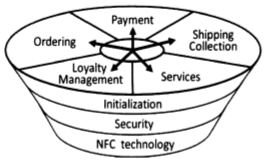
\includegraphics[width=0.5\textwidth]{nmcModel.png}
      \caption{El modelo \acs{NMC}.}
      \label{fig:nmcModel}
    \end{center}
  \end{figure}

  \begin{itemize}
  \item \textbf{Fase de inicialización}. Para la construcción de un servicio
  de comercio basado en \acs{NFC} se necesitan definir cuatro componentes
  fundamentales:
    \begin{itemize}
    \item \textbf{Servicio de \emph{back-end}}\footnote{En diseño de software
    el \emph{front-end} es la parte del software que interactúa con el o los
    usuarios y el \emph{back-end} es la parte que procesa la entrada desde el
    \emph{front-end}} \textbf{basado en \acs{NFC}}. Este
    servicio es el responsable de todo el intercambio de información durante
    el proceso de comercio. Está gestionado por el proveedor de servicios
    basados en \acs{NFC}.
    \item \textbf{Aplicación de terminal genérico (\acs{GTA})}. Como el tamaño
    de la memoria del dispositivo móvil es limitada, combiene definir una
    aplicación genérica que permita realizar todas las gestiones comerciales.
    \item \textbf{Funcionalidad de las etiquetas}. Definir los tipos de
    etiquetas que se utilizarán para construir un entorno de servicios con
    \acs{NFC} que siga el estándar \acs{NDEF}. Por ejemplo, un tipo de etiqueta
    para iniciar la aplicación, otro para cada uno de los productos, otro
    para seleccionar descuentos y otro para seleccionar el servicio.
    \item \textbf{Habilitar el servicio \acs{NFC}}. La etiqueta de inicio de
    aplicación se encargará de cargar el \acs{GTA} y de arrancar el servicio de
    \emph{back-end}, para que el usuario pueda usarlos nada más iniciar la
    aplicación.
    \end{itemize}
  \item \textbf{Fase de pedido}. Después de la inicialización el cliente ya
  está preparado para realizar un pedido a través de un catálogo de productos:
    \begin{itemize}
    \item Cada \textbf{catálogo} tiene una o varias etiquetas que representan
    los productos ofrecidos por el servicio. Cuando el dispositivo toca una
    de estas etiquetas, la aplicación puede llamar al servicio \emph{back-end}
    para descargar el contenido (imágenes, videos, etc.) relacionado con el
    contenido del producto al que representa la etiqueta.
    \item Además, cada producto puede tener opciones del tipo \emph{sabor},
    \emph{volumen}, \emph{tamaño}; que pueden ser seleccionables a través
    de otras etiquetas o a través de la pantalla del dispositivo.
    \end{itemize}
  \item \textbf{Fase de pago}. Hay dos métodos de pago disponibles en el
  modelo \acs{NMC}:
    \begin{itemize}
    \item \textbf{Modo monedero electrónico} (figura \ref{fig:e-wallet}). 
    Después de que el cliente haya realizado un pedido, el \acs{GTA} 
    solicitará la información del producto al servicio \emph{back-end}. Si el 
    servicio \emph{back-end} confirma la autenticidad del usuario y de la 
    operación, le devolverá al \acs{GTA} el importe del producto. Esta 
    cantidad será decrementada del monedero electrónico. El monedero 
    electrónico es un elemento seguro al que sólo se puede acceder con el 
    permiso del servicio \emph{back-end}. Los clientes deben disponer de saldo 
    para poder realizar un pedido (método prepago).

    \begin{figure}[!h]
      \begin{center}
        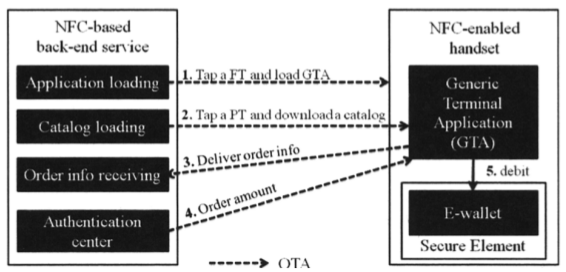
\includegraphics[width=0.5\textwidth]{e-wallet.png}
        \caption{Fase de pago con \emph{modo monedero electrónico}.}
        \label{fig:e-wallet}
      \end{center}
    \end{figure}

    \item \textbf{Modo tarjeta de crédito} (figura \ref{fig:creditCard}). 
    Antes de utilizar este modo para llevar a cabo la transacción, el banco 
    debe facilitar al cliente un \emph{applet\footnote{Componente de una 
    aplicación que se ejecuta en el contexto de otro programa. No puede 
    ejecutarse de manera independiente.}} que tiene que ser cargado en el 
    dispositivo móvil. Una vez realizado el pedido, el \acs{GTA} almacena el 
    número de orden como elemento seguro. Para realizar el pago, el cliente 
    aproxima el dispositivo móvil al lector del comerciante y este lee el 
    número de orden almacenado. El servicio de \emph{back-end} comprueba el 
    importe a pagar y se inicia un intercambio de información entre el lector 
    del banco y el \emph{applet} de la tarjeta de crédito. Por último, el 
    lector del banco obtiene el código de autorización para finalizar la 
    transacción.
  
    \begin{figure}[!h]
      \begin{center}
        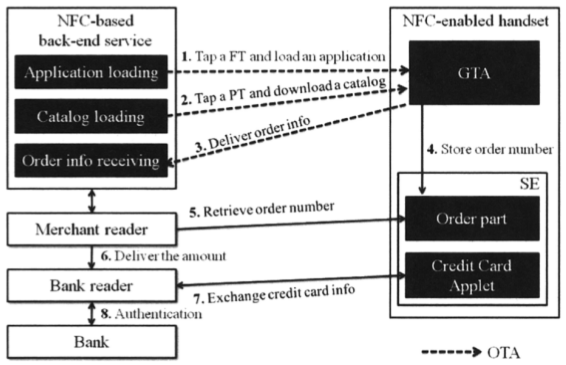
\includegraphics[width=0.5\textwidth]{creditCard.png}
        \caption{Fase de pago con \emph{modo tarjeta de crédito}.}
        \label{fig:creditCard}
      \end{center}
    \end{figure}

    \end{itemize}
  \item \textbf{Fase de envío y recogida}. En esta fase, el cliente elige
  la forma y el lugar en que recibe el producto o servicio. Para productos
  físicos elegirá el lugar al que deben llevárselo o el lugar en el que quiere
  recogerlo. Y para productos virtuales el dispositivo donde quiere
  almacenarlo.
  \item \textbf{Fase de gestión de fidelización}. El programa de fidelización
  está diseñado para incentivar al cliente a consumir de nuevo. Los cupones son
  herramientas de fidelización comunes y la tecnología \acs{NFC} hace factible
  el concepto de \emph{cupones virtuales}.
    \begin{itemize}
    \item Los clientes pueden recibir cupones tocando una etiqueta que 
    simbolice la descarga de un cupón.
    \item A través de \acs{NFC}, utilizando el modo de comunicación
    \emph{peer-to-peer}, los clientes pueden compartir sus cupones con los
    demás. Esto puede aprovecharse para desarrollar un programa de
    \emph{márketing} atractivo y eficaz.
    \end{itemize}
  \item \textbf{Fase de servicio}. Para solicitar un servicio bastará con
  tocar con el dispositivo móvil una etiqueta de tipo servicio. Las diferentes
  opciones de servicio que estén disponibles serán accesibles a través de
  otras etiquetas de servicio o mediante la selección de ese servicio en la
  pantalla del dispositivo.
  \end{itemize}
  
  Dada su generalidad, el modelo basado en el comercio móvil \acs{NMC} está 
  pensado para establecer las líneas maestras a la hora de desarrollar 
  cualquier clase de servicios móviles; entre ellos por supuesto, un sistema
  de gestión de restaurantes basado en \acs{NFC}.

    \subsubsection{Métodos de pago móvil a distancia}
  Hoy en día se pueden distinguir dos tipos de pagos a distancia: los que se
  producen de forma remota, como cuando se realizan compras por internet;
  y los que se realizan dentro del mismo sitio donde se está
  comprando. El primero de ellos goza de una gran popularidad, ya que se
  considera un método fácil, cómodo y bastante seguro; y no requiere de una
  infraestructura especial para ser implementado. El segundo en cambio,
  aún no goza de la misma aceptación, debido en parte a que los 
  establecimientos no están dispuestos a invertir su dinero en adquirir una 
  infraestructura adicional para permitir este tipo de pagos, sin ver antes 
  que hacerlo les reporte algún tipo de beneficio.

  En la actualidad el pago a distancia por móvil utilizando la tecnología
  \acs{RFID} y \acs{NFC} se puede conseguir mediante uno de estos tres métodos:
  \begin{description}
  \item[SIMpass]. Es una tecnología de interfaz dual que combina la
  tradicional tarjeta \acs{SIM} y la tarjeta \acs{RFID}, en una sola tarjeta
  estándar. La interfaz de contacto cumple con la norma \acs{ISO} 7816 y la
  interfaz a distancia cumple con el estándar de la norma \acs{ISO} 14443.
  \emph{SIMpass} trabaja con una frecuencia de 13,56MHz. Como no es una
  frecuencia muy alta, es difícil minimizar el tamaño de antena. Existen dos
  maneras de implementar dicha antena. Una, de bajo coste, se lleva a cabo 
  utilizando una antena plana que consta de una bobina y que se une a la 
  del teléfono móvil. Para la otra, hay que reformar parte del hardware del 
  teléfono móvil, aunque mejora notablemente la estabilidad y fiabilidad de la
  funcionalidad \acs{RFID}.

  \item[NFC]. Como se ha visto en secciones anteriores, \acs{NFC} es una
  tecnología que combina la tecnología \acs{RFID} con las comunicaciones de
  corto alcance. En el sistema \acs{NFC} propuesto se distinguen tres partes 
  principales: el controlador, la antena y una unidad de seguridad. La unidad
  de seguridad puede correr a cargo de la tarjeta \acs{SIM} o de la tarjeta
  \acs{SD}. El problema está en que, tanto en un caso como en otro, habría que 
  integrar un módulo o chip de seguridad que no viene por defecto en estas 
  tarjetas. Esto se soluciona utilizando la tecnología \acs{NFC} mejorada 
  (\emph{eNFC}). Aunque \emph{eNFC} hace uso de la tarjeta \acs{SIM}, sólo 
  tiene que utilizar el pin C6 para poder modificar la memoria \emph{EEPROM}, 
  en vez de tener que utilizar dos pines (C4 y C8) que además interferirían a 
  la hora de realizar otras operaciones.

    \item[Programa RF-SIM]. Combinando el módulo de comunicaciones móviles y
  los micro-módulos de radio frecuencia (\emph{RF}) de la tarjeta \acs{SIM}
  normal, la tarjeta \emph{RF-SIM} consigue operar a 2,4GHz (una alta 
  frecuencia que tiene una longitud de onda corta). Esto permite que, a través
  de una antena, el módulo \emph{RF-SIM} pueda comunicarse con otros 
  dispositivos externos a distancias entre los 10 y los 500cm, a pesar de que
  dicho módulo tenga un tamaño muy reducido. \emph{RF-SIM} es un tipo de
  etiqueta activa, por lo que necesita una batería para trabajar.
  \end{description}

%%%%%%%%%%%%%%%%%%% He leído hasta aquí %%%%%%%%%%%%%%%%%%%%%%%%%%%%%%%%
%%%%%%%%%%%%%%%%%%%%%%%%%%%%%%%%%%%%%%%%%%%%%%%%%%%%%%%%%%%%%%%%%%%%%%%%

  Cada uno de estos métodos tiene sus ventajas e inconvenientes. Por ejemplo:
  \begin{itemize}
  \item Para implementar el método \emph{SIMpass} es necesario utilizar los
  pines \emph{C4} y \emph{C8}, que están reservados para la interfaz de alta
  velocidad de la tarjeta \acs{SIM}. Por lo tanto tiene un conflicto en la
  evolución futura de la tarjeta \acs{SIM}. Además, aunque la antena que
  necesita tiene un costo más asequible; la fiabilidad, el alcance y la
  velocidad de las transacciones dejan mucho que desear. Por lo que se 
  considera un método poco recomendable.
  \item La distancia de reacción es el factor más significativo de un sistema
  \acs{RFID}. Para un sistema de pago, cuanto más corta sea esta distancia
  más segura será la transacción. El programa \emph{RF-SIM} trabaja a 2.4GHz,
  lo que implica que la distancia de reacción sea demasiado larga como para ser
  segura. Los sistemas inalámbricos \emph{Bluetooth}, \emph{Zigbee}
  \footnote{Especificación de un conjunto de protocolos de alto nivel de 
  comunicación inalámbrica para su utilización con radiodifusión digital de 
  bajo consumo, basada en el estándar IEEE 802.15.4 de redes inalámbricas de 
  área personal. Su objetivo son las aplicaciones que requieren comunicaciones 
  seguras con baja tasa de envío de datos y maximización de la vida útil de 
  sus baterías, como las aplicaciones domóticas.},
  \acs{WiFi} o \acs{UWB}\footnote{Cualquier tecnología de radio que usa un
  ancho de banda mayor de 500 MHz o del 25\% de la frecuencia central, de 
  acuerdo con la FCC (Federal Communications Commission).} usan la misma 
  frecuencia, lo que puede generar interferencias.
  \item El sistema \emph{NFC-SIM} tiene el mismo problema con los pines que
  \emph{RF-SIM} y \emph{NFC-SD} es una solución demasiado costosa.
  \item \emph{eNFC} se plantea como la solución óptima para resolver todos los
  problemas.
  \end{itemize}

  Como se decía, aunque muchos analistas e ingenieros hablan de que los 
  pagos mediante \acs{NFC} sustituirán a los pagos realizados por medios
  tradicionales, esta tecnología aún no es muy común en los teléfonos. En
  Estados Unidos, sólo dos modelos han incluido el hardware \acs{NFC}
  que soporta el pago mediante \emph{Google Wallet}\footnote{Sistema de pago 
  móvil desarrollado por \emph{Google} que permite a los usuarios guardar las 
  tarjetas de crédito, tarjetas de fidelización y tarjetas de regalo, entre 
  otras cosas. Soporta el uso de \acs{NFC}.}. En 2012 se ha anunciado
  la salida de más de 100 modelos con funcionalidad \acs{NFC} (doblando las 
  cifras del 2011). Pero sólo con la producción de más teléfonos con \acs{NFC} 
  no es suficiente. Las tiendas tienen que añadir lectores \acs{NFC} a todas
  sus cajas registradoras y los minoristas no quieren gastar dinero en esto
  hasta que la demanda no sea significativa. Por ello, mientras que esto 
  ocurre, han aparecido nuevas formas de pago que aprovechan las 
  características de otras tecnologías con las que cuentan los móviles, como 
  la lectura de códigos \acs{QR}, el acelerómetro o mediante
  \acs{SMS}\cite{bib:noWaiting}.

    \subsubsection{Métodos de fidelización de clientes}
  Uno de los atractivos que puede tener el uso de la tecnología móvil \acs{NFC}
  es el de poder fidelizar a los clientes en el uso de un servicio. Para ello,
  dependiendo de las operaciones realizadas en el
  establecimiento, este puede ofrecerle productos que tal vez le interesen,
  puede proponerle descuentos por su fidelidad como cliente o puede utilizar
  el historial de todos los clientes para conocer cuáles son las tendencias
  de consumo.
  
  Uno de los últimos sistemas propuestos para sacar 
  partido a la utilización del \acs{NFC} es \emph{\textbf{WingBonus}}.

  \emph{\href{http://wingbonus.com/}{WingBonus}} es un sistema de
  gestión de promociones formado por una aplicación web y una aplicación móvil
  (disponible para sistemas \emph{Android}). Ha sido creada por el grupo de 
  investigación ISCBD (Ingeniería del Software, Conocimiento y Base de datos) 
  de la Universidad de Córdoba. Y, aunque por el momento sólo muestra 
  promociones ficticias, tiene por objetivo servir algún día de punto de 
  encuentro entre los clientes y sus marcas favoritas, a través de las 
  promociones ofertadas por estos últimos.
  
  A través de la web, los clientes pueden descargar en su móvil cupones, 
  descuentos o tarjetas de fidelización, que pueden ser utilizados a la hora 
  de realizar un pago con \acs{NFC} en los establecimientos donde tengan 
  vigencia. Es decir, si un cliente tiene un cupón de descuento para cortarse 
  el pelo en una peluquería concreta y al pagar en dicha peluquería utiliza el 
  sistema \acs{NFC}, el precio total a abonar por el corte de pelo se verá 
  decrementado por el cupón de descuento.

  El sistema permite dos tipos de usuarios: el usuario registrado y el usuario
  anónimo. Los cupones disponibles para cata tipo de usuario presentan
  características diferentes. Por ejemplo, habrá cupones en los que las
  empresas se interesen por conocer qué tipo de personas (edad, trabajo,
  estatus, etc) descargan y utilizan este tipo de cupones. Si la empresa no
  se preocupa por esta información, todo el mundo podrá descargar cupones
  como anónimo.

  Todas las ofertas que se ofrecen en la web tienen un periodo concreto de
  disponibilidad dentro del cual el cliente puede hacerse con dicha oferta
  (figura \ref{fig:wingBonusP}). Además, las ofertas tienen un tiempo acotado
  de validez que delimita el periodo en el que puede aplicarse dicha oferta.

  \begin{figure}[!h]
    \begin{center}
      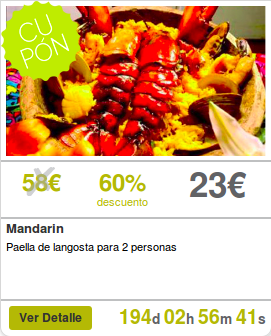
\includegraphics[width=0.5\textwidth]{wingBonusP.png}
      \caption{Ejemplo de cupón ofrecido en la web de \emph{WingBonus}.}
      \label{fig:wingBonusP}
    \end{center}
  \end{figure}

  Los cupones de descuentos tienen la particularidad de que pueden compartirse
  con otros usuarios \acs{NFC} mediante una comunicación \emph{peer-to-peer}.

  Para las empresas asociadas, \emph{WingBonus} ofrece grandes ventajas: 
  reducción de costos, eliminación del papel, poder llegar a más clientes,
  eliminación de las falsificaciones, análisis de mercado, estudio de
  tendencias, fidelización de clientes, etc.\cite{bib:wingBonus}.

  \subsection{Aplicaciones comerciales}
  A continuación, se muestran varios ejemplos de cómo distintos programas
  comerciales implementan las funcionalidades típicas de los gestores de
  restaurantes. Después, se expondrán algunas aplicaciones que permiten
  realizar pedidos desde el sitio sin necesidad de tener que avisar al
  camarero.

    \subsubsection{Gestión de operaciones típicas de un restaurante}
    En la actualidad existe una innumerable oferta de aplicaciones que ayudan
    a gestionar las labores típicas de un restaurante, como pueden ser:
    gestionar pedidos, generar facturas o realizar la función de caja 
    registradora.

    \begin{itemize}
    \item Para \textbf{gestionar pedidos} las aplicaciones suelen contar con 
    un panel de productos en el que se van seleccionando: cantidad, producto y 
    mesa a la que va destinado (figuras \ref{fig:productsPanel} y
    \ref{fig:productsPanel2}). Normalmente la iteración consiste en: primero,
    seleccionar una mesa; después, seleccionar la cantidad; y por último,
    seleccionar el producto.

    \begin{figure}[!h]
      \begin{center}
        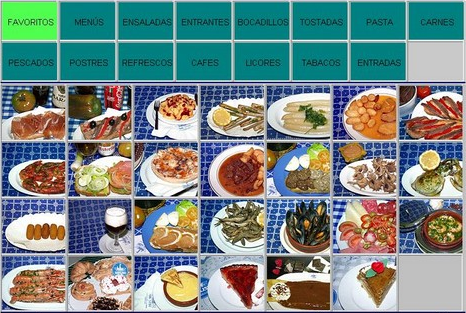
\includegraphics[width=0.8\textwidth]{productsPanel.png}
        \caption{Panel de productos del programa \emph{FrontRest}
        \cite{bib:frontRest}.}
        \label{fig:productsPanel}
      \end{center}
    \end{figure}

    \begin{figure}[!h]
      \begin{center}
        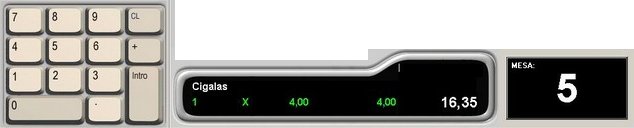
\includegraphics[width=0.8\textwidth]{productsPanel2.png}
        \caption{Panel de selección de cantidad del programa \emph{FrontRest}
        \cite{bib:frontRest}.}
        \label{fig:productsPanel2}
      \end{center}
    \end{figure}

    Una vez terminada la iteración anterior, el pedido queda reflejado en la
    lista de productos asignados a esa mesa (figura \ref{fig:productsList}).

    \begin{figure}[!h]
      \begin{center}
        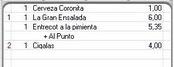
\includegraphics[width=0.5\textwidth]{productsList.png}
        \caption{Lista de pedidos para la mesa 5. \emph{FrontRest}
        \cite{bib:frontRest}.}
        \label{fig:productsList}
      \end{center}
    \end{figure}

    \item A la hora de \textbf{facturar una mesa}, este tipo de aplicaciones 
    suelen presentar un resumen con los datos de la mesa a facturar, la lista 
    de pedidos realizados, el importe parcial de cada uno de ellos, el importe
    subtotal y el importe total con impuestos incluidos (figura
    \ref{fig:bill}).

    \begin{figure}[!h]
      \begin{center}
        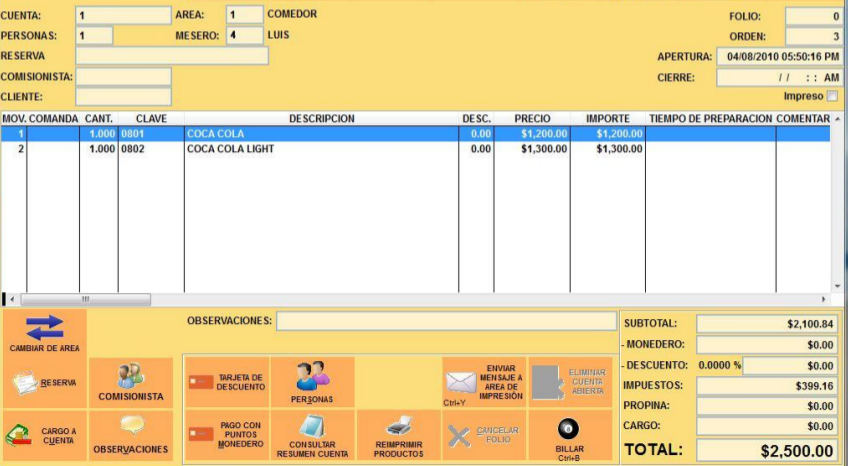
\includegraphics[width=1\textwidth]{bill.png}
        \caption{Resumen de facturación de una mesa en el programa
        \emph{Soft Restaurant}\cite{bib:softRestaurant}.}
        \label{fig:bill}
      \end{center}
    \end{figure}

    Con estos datos, el camarero conoce en tiempo real cuál es la lista de
    productos de una mesa y cuál es el importe total que los comensales deben
    abonar en concepto de los productos consumidos.

    \item Los \textbf{productos} con los que estos programas trabajan, deben 
    ser editados por los responsables del restaurante. Entre los atributos que
    estos poseen están: código, nombre, categoría o precio (figura
    \ref{fig:editProduct}).

    \begin{figure}[!h]
      \begin{center}
        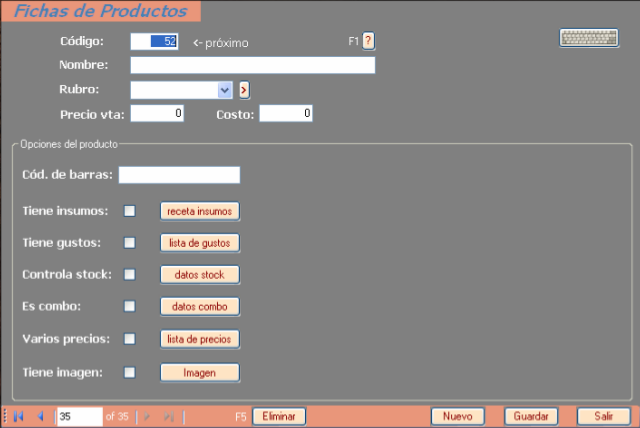
\includegraphics[width=0.8\textwidth]{editProduct.png}
        \caption{Editor de productos del programa \emph{SaleYa}
        \cite{bib:saleYa}.}
        \label{fig:editProduct}
      \end{center}
    \end{figure}
    \end{itemize}

    Estas son las funcionalidades básicas que todo software de 
    gestión de restaurante debe tener. Pero, aparte de estas, son muchas otras 
    las funcionalidades que pueden ayudar a mejorar la gestión de un 
    restaurante.

    \begin{itemize}
    \item Es muy común en casi todos los programas de gestión de restaurantes
    buscar una \textbf{representación aproximada de las partes que forman el
    restaurante}. En un principio, lo que más interesa es representar las 
    mesas del restaurante, aunque hay aplicaciones que representan también
    la barra, las mesas del salón, las mesas de la terraza y otros objetos
    (figura \ref{fig:tables}).

    \begin{figure}[!h]
      \begin{center}
        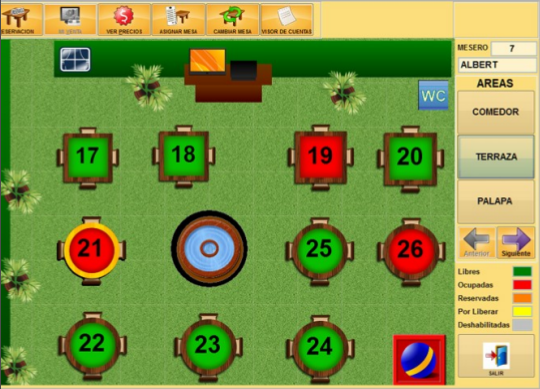
\includegraphics[width=0.8\textwidth]{tables.png}
        \caption{Mapa de un restaurante de la aplicación
        \emph{Soft Restaurant}\cite{bib:softRestaurant}.}
        \label{fig:tables}
      \end{center}
    \end{figure}

    Estos mapas ayudan a los camareros a reconocer el estado en el que se
    encuentran las mesas (ocupadas, libres, reservadas, deshabilitadas, etc.).
    Los símbolos del mapa ayudan a ubicar dónde se encuentran los objetos
    reales a los que representan y su color representa el estado en el que
    se encuentran.

    \item Aplicaciones como \emph{Soft Restaurant}\cite{bib:softRestaurant} o 
    \emph{SaleYa}\cite{bib:saleYa} tienen una funcionalidad que permite 
    \textbf{describir las recetas} de los productos contemplados en la carta. 
    Es decir, permite listar los ingredientes (con sus cantidades) utilizados 
    en la elaboración de cada plato (figura \ref{fig:ingredients}). Esto 
    facilita la gestión del \emph{stock} de dichos ingredientes.

    \begin{figure}[!h]
      \begin{center}
        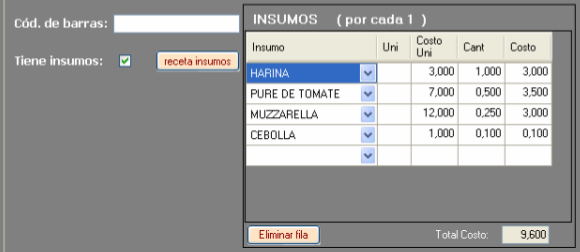
\includegraphics[width=0.8\textwidth]{ingredients.png}
        \caption{Ingredientes para la elaboración de una \emph{pizza de 
        mozzarella}. \emph{SaleYa}\cite{bib:saleYa}.}
        \label{fig:ingredients}
      \end{center}
    \end{figure}

    Esta funcionalidad ayuda a los cocineros y a sus ayudantes a conocer
    mejor cuáles son los ingredientes necesarios para la elaboración de 
    un plato y les ayuda a gestionar de una manera más eficiente el
    \emph{stock} de los ingredientes, según las necesidades que la 
    elaboración cada plato demande.

    \item Una funcionalidad que puede ser muy útil a la hora de gestionar
    los pedidos es incorporar un terminal en la cocina, para que los cocineros
    informen del \textbf{estado de preparación de las comandas} (figura
    \ref{fig:kitchen}).

    \begin{figure}[!h]
      \begin{center}
        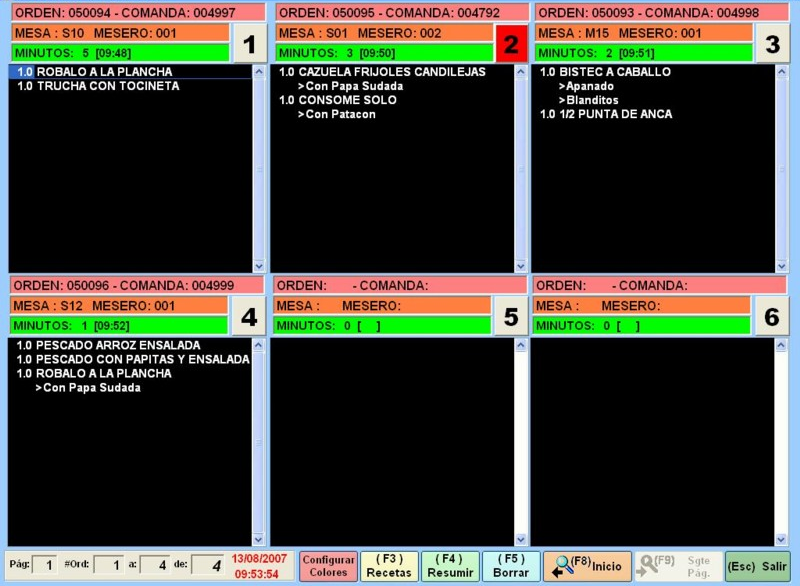
\includegraphics[width=0.8\textwidth]{kitchen.png}
        \caption{Monitor de comandas de la aplicación \emph{RestBar}
        \cite{bib:restBar}.}
        \label{fig:kitchen}
      \end{center}
    \end{figure}
    
    La aplicación muestra qué camarero ha solicitado el plato, la hora en que
    lo solicitó y los minutos que han pasado desde que lo hizo. Cuando los
    productos están listos para servir, los cocineros informan a los
    camareros, cambiando el estado del pedido a través de la aplicación.

    \item Si el restaurante tiene entre sus servicios el \textbf{reparto a
    domicilio}, no está demás que la aplicación cuente con una funcionalidad
    en la que quede constancia de los pedidos a domicilio que tiene pendientes
    (figura \ref{fig:deliveries}):

    \begin{figure}[!h]
      \begin{center}
        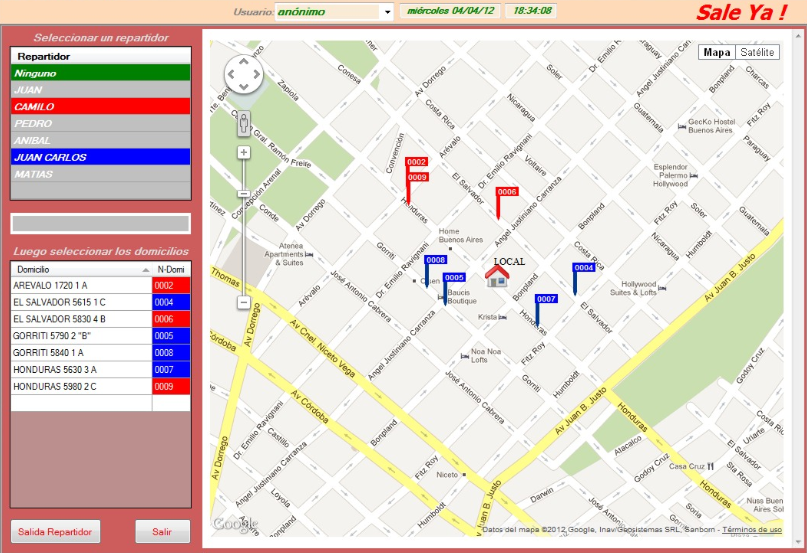
\includegraphics[width=0.8\textwidth]{deliveries.png}
        \caption{Módulo que gestiona los repartos a domicilio. \emph{SaleYa}
        \cite{bib:saleYa}.}
        \label{fig:deliveries}
      \end{center}
    \end{figure}

    La aplicación registra cuáles son los pedidos pendientes, qué repartidor
    se encargará de atenderlos y dónde están los puntos de entrega.
    \end{itemize}

    El abanico de programas de gestión de restaurantes es muy diverso. A la
    hora de adquirir uno u otro conviene determinar bien qué necesidades de
    información se deben satisfacer, de tal forma que no se eche en falta 
    ninguna funcionalidad y que no se tengan funcionalidades incompatibles
    con el modelo de negocio que se posee.

    \subsubsection{Gestión de pedidos a través de dispositivos móviles}
    Las soluciones vistas en el apartado anterior van encaminadas a
    facilitar las tareas propias de los camareros y cocineros del restaurante,
    pero en ninguna de ellas se tiene en cuenta al cliente. Si el cliente es
    capaz de realizar pedidos sin necesidad de avisar a un camarero, este
    quedará liberado para realizar otras tareas.

    A continuación, se presentan dos soluciones comerciales que buscan
    satisfacer este objetivo:

    \begin{itemize}
    \item \textbf{vMenu}. Es un sistema ideado por la empresa \emph{Vloo} que
    trata de reinventar la carta tradicional adentrándose en el mundo
    interactivo actual, a través de las pantallas táctiles. Los clientes
    disponen de un dispositivo (\emph{iPad}, tablet o pantalla) en la que
    pueden ver los platos disponibles y realizar los pedidos (figura
    \ref{fig:starters}).

    \begin{figure}[!h]
      \begin{center}
        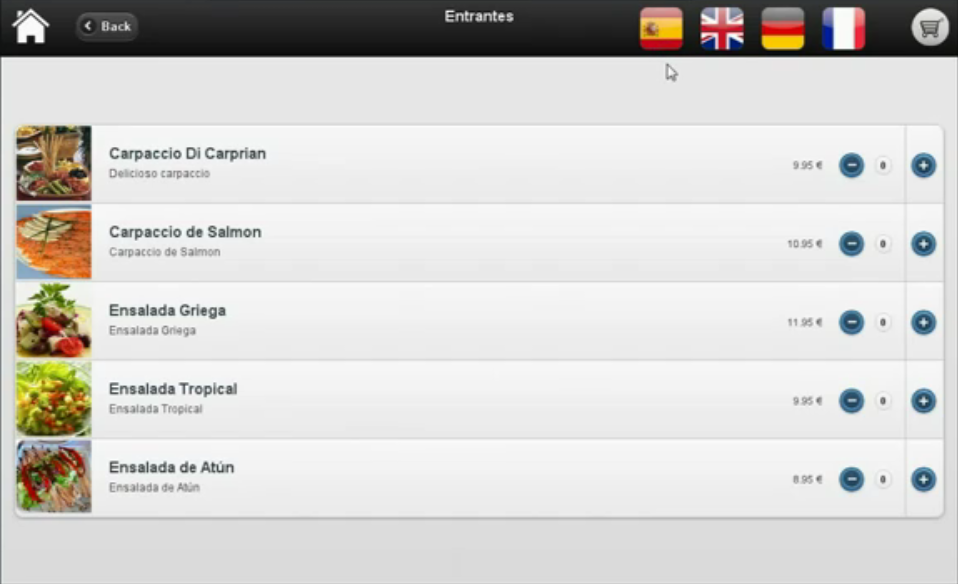
\includegraphics[width=0.8\textwidth]{starters.png}
        \caption{Lista de productos \emph{entrantes}.}
        \label{fig:starters}
      \end{center}
    \end{figure}

    Los productos aparecen distribuidos por categorías y son actualizados
    de manera instantánea. Además, los alimentos son mostrados de una forma
    más atractiva: con fotos, ingredientes, recetas, calorías, preparación y 
    otros datos de interés; y siempre en el idioma del comensal (figura
    \ref{fig:meat}).

    \begin{figure}[!h]
      \begin{center}
        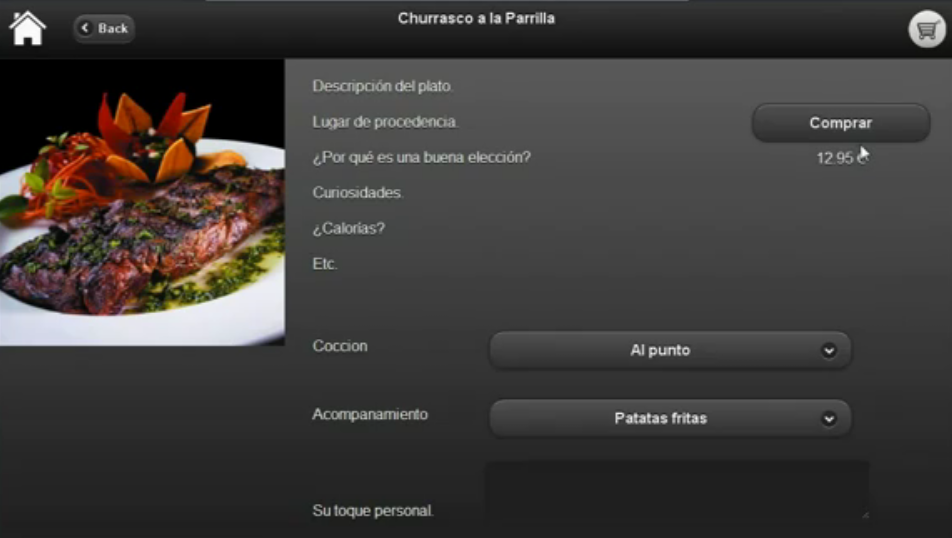
\includegraphics[width=0.8\textwidth]{meat.png}
        \caption{Información asociada al \emph{churrasco a la parrilla}.}
        \label{fig:meat}
      \end{center}
    \end{figure}
    
    \emph{vMenu} reduce los tiempos de espera porque el cliente no necesita
    al camarero para conocer los productos, las recomendaciones o las ofertas
    disponibles; ni para realizar el pedido (figura \ref{fig:order}) o
    solicitar la cuenta; y en caso de necesitarlo, dispone de una opción para
    llamarlo desde el terminal.

    \begin{figure}[!h]
      \begin{center}
        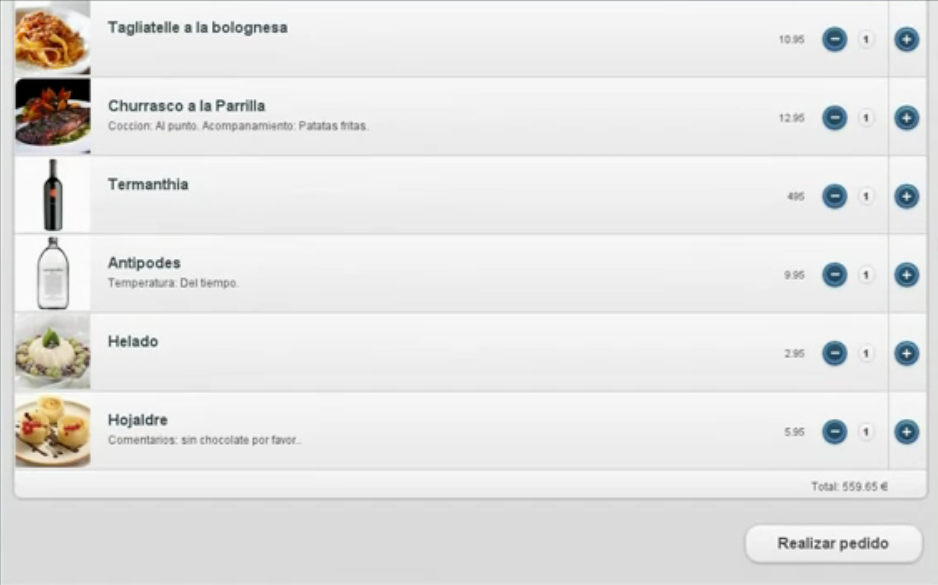
\includegraphics[width=0.8\textwidth]{order.png}
        \caption{Lista de productos elegidos para un pedido.}
        \label{fig:order}
      \end{center}
    \end{figure}

    Por último, a parte de esta función de recogida de pedidos, \emph{vMenu} 
    dispone de todo un sistema integral que permite gestionar las operaciones
    básicas de un restaurante\cite{bib:VMENU}.

    \item \textbf{Brand Table}. \emph{S-Digital}, una \emph{start-up} de la
    Universidad de Sidney, ofrece este prototipo conceptual de mesa de
    restaurante en torno a la cual se distribuyen varios menús electrónicos con
    los que se puede interactuar utilizando un dispositivo móvil con \acs{NFC}
    (figura \ref{fig:brandTable}), de forma que los comensales que se reúnan a 
    su alrededor puedan seleccionar su comida favorita y pagarla
    \emph{in situ} (utilizando \emph{Google Wallet} o \emph{Paypal Mobile}), 
    sin necesidad de tener que esperar a ningún camarero que les tome nota del 
    pedido (figura \ref{fig:brandTableDemo}).

    \begin{figure}[!h]
      \begin{center}
        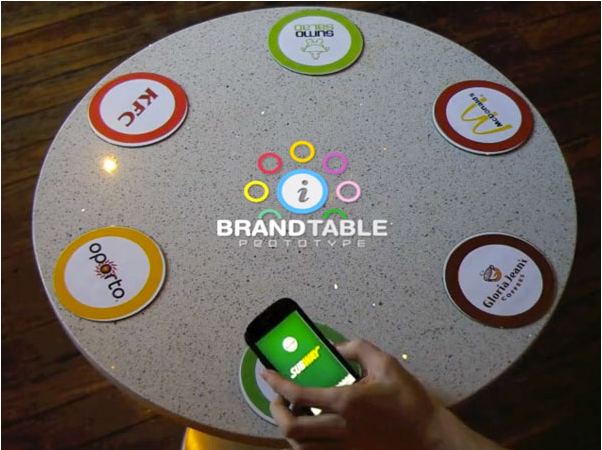
\includegraphics[width=0.8\textwidth]{brandTable.png}
        \caption{Prototipo conceptual de la mesa \emph{Brand Table}.}
        \label{fig:brandTable}
      \end{center}
    \end{figure}

    \begin{figure}[!h]
      \begin{center}
        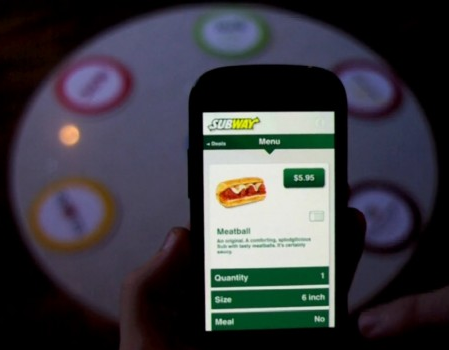
\includegraphics[width=0.8\textwidth]{brandTableDemo.png}
        \caption{Selección de uno de los productos del restaurante
        \emph{Subway}.}
        \label{fig:brandTableDemo}
      \end{center}
    \end{figure}

    Cuando el pedido está preparado, el cliente se levanta y va a recogerlo.
    
    Este sistema está pensado para restaurantes de comida rápida y elimina
    completamente la labor del camarero\cite{bib:brandTable}.
    \end{itemize}


% Local Variables:
%   coding: utf-8
%   mode: latex
%   mode: flyspell
%   ispell-local-dictionary: "castellano8"
% End:
